%%%%%%%%%%%%%%%%%%%%% chapter2.tex %%%%%%%%%%%%%%%%%%%%%%%%%%%%%%%%%
%
%  Monotone Circuits Lower bounds 
%
% Use this file as a template for your own input.
%
%%%%%%%%%%%%%%%%%%%%%%%% Springer-Verlag %%%%%%%%%%%%%%%%%%%%%%%%%%
%\motto{Use the template \emph{chapter.tex} to style the various elements of your chapter content.}





\chapter{Monotone Circuit Lower Bounds}
\label{sec:Razborov} % Always give a unique label
% use \chaptermark{}
% to alter or adjust the chapter heading in the running head


% Always give a unique label
% and use \ref{<label>} for cross-references
% and \cite{<label>} for bibliographic references
% use \sectionmark{}
% to alter or adjust the section heading in the running head

We've seen that proving that SAT is not in $P/poly$, i.e., can't be solved by polynomial-size circuits, implies that $P \neq NP$.
Due to the notorious difficulty of these questions, we are interested in proving \emph{weaker} lower bounds, namely, some lower bounds against restricted classes of circuits. 
Here, we study such a restricted circuit class: A boolean circuit without negation gates, i.e., monotone circuits.

\begin{definition}[Monotone circuit]
A Monotone circuit is a Boolean circuit that contains fan-in two gates AND and OR, but has \emph{no} NOT gates.
\end{definition}

This means in particular that monotone circuits can compute only monotone functions: a Boolean function is said to be monotone if increasing the number of ones in the input cannot flip the value of the function from 1 to 0. 

More precisely, for $\bar{x}, \bar{y} \in\{0,1\}^n$, write $\bar{x} \geqslant \bar{y}$ iff $ \forall i \in [n], x_i \geqslant y_i$, where $[n]$ denotes $\{1,\dots,n\}$. (Here, $x_i\ge y_i$ for Boolean $x_i,y_i$ means simply that $1\ge 0$ and $0\ge 0$, $1\ge 1$, while $0\not\ge 1$.)

\begin{definition}[Monotone function]
A Boolean function $f:\{0,1\}^n \rightarrow\{0,1\}$ is said to be  \emph{monotone} if $\forall \bar{x} \geq \bar{y}, f(\bar{x}) \geqslant f(y)$.
\end{definition}


Many NP problems are monotone, like CLIQUE:

Given an undirected graph $G=(V, E)$ with $n$ nodes, a $k$-clique in $G$ is a set $U\subseteq V$ of size $k$, st. every pair of nodes $u_1, u_2 \in U$ is connected by an edge (in $E$):

$$
 \forall u_1 \in u \forall u_2 \in u ( u \neq u_2\Rightarrow (u_1, u_2)\in E).
$$


Recall that a computational (decision) problem is a \emph{language}, namely an infinite set of finite strings over a finite alphabet (usually the alphabet $\{0,1\}$). Here, our language consists of all the strings that encode (in some natural way) an accepted graph, i.e., a $k$-clique with $n$ nodes.
The natural way to encode a graph in our case is this: a graph  $G=(V, E) $ w / $n$ nodes, is encoded by $\binom{n}{2}$ input variables  $x_{ij}$, where the semantic of the encoding is: $x_{i j}=1$ iff $(i, j) \in E$. In other words, if the input variable $x_{ij}=1$,   our input graph contains the edge $(i,j)$, and otherwise it does not. 

We are interested in CLIQUE $(k, n)$ for a fixed $k$, as the following Boolean function: 
\begin{svgraybox}
The computational problem \textbf{CLIQUE $(k, n)$:}  

Input: Graph w/ $n$ nodes and a number $k$

Accept if the graph contains a $k$-clique. Reject otherwise.
\end{svgraybox}


 Note that $\operatorname{CLIQUE}(k, n)$ is a monotone function: If we add 1's to the input, we only \emph{increase} the chance it has a $k$-clique!
 
It is known that CLIQUE$(k,n)$ is NP-complete (see standard complexity textbooks; e.g., Papadimitriou 1994).


Since CLIQUE$(n, k)$ is a monotone (Boolean)
function we can compute it by a monotone Boolean circuit.
\medskip 

\textbf{Example of a monotone circuit computing CLIQUE$(n, k)$:} ``run" over all $\binom{n}{k} ~~ k$-sub-graphs in $G$, and check if at least one of those is a clique:

\begin{figure}
    \centering
    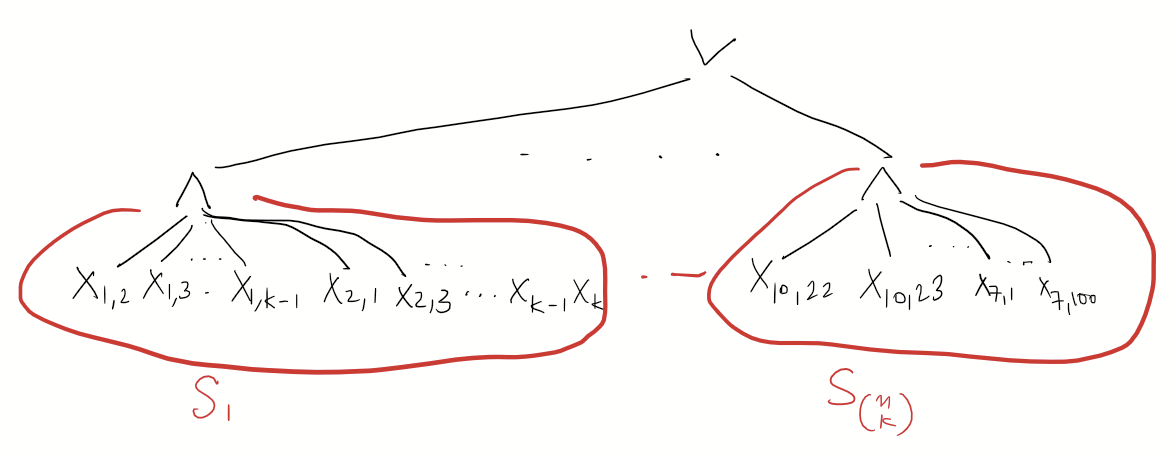
\includegraphics[width=0.75\linewidth]{images/k-clique-simple-circuit.png}
    \label{fig:enter-label}
\end{figure}





$S_1, S_2, \ldots, S_{\binom{n}{k}}$ are the $\binom{n}{k}$ subgraphs in $G$ each of size $k$.
Size of this circuit: $O\left(k^2 \cdot\binom{n}{k}\right)$.
We call such a circuit for computing $\operatorname{CLIQUE}  (n, k)$ consisting of a big $\lor$ of all $S_i$'s, each computed by $\land$'s of edges, a \textbf{\textit{crude-circuit}} for CLIQUE($n, k)$.


Notation: $CC\left(S_1, \ldots, S_{\binom{n}{k}}\right)$ is the crude circuit computing the $\lor$ of all subgraphs $S_1 \ldots S_{n\choose k }$. In general, we shall use different subgraphs: $CC\left(x_1, \ldots, x_m\right)$ for $x_i \subseteq V$ not necessarily of size $k$.


Note: When $k=w(\log n)$, $CC\left(S_1, \ldots, S_{\left(k_k\right)}\right)$ is of exponential size.
The following theorem shows this naive monotone circuit cannot be improved much:

\begin{figure}
    \centering
    
\includegraphics[width=0.25\linewidth]{images/RAZBOROV_Alexander.jpeg}
    \caption{Enter Caption}
    \label{fig:enter-label}
\end{figure}


\begin{theorem}
    [Razborov] Let $k=\sqrt[4]{n}$. Then every monotone circuit computing CLIQUE$(n, k)$ has size $2^{\Omega(\sqrt[8]{n})}$.
\end{theorem}
That is, exists a constant $c$ s.t. for large enough $n \in \mathbb{N}$, if $C_n$ computes CLIQUE$(n,k)$ then $\left|C_n\right| \geqslant 2^{c \cdot \sqrt[8]{n}}$.


%Recall: a crude circuit is a big OR of cliques, each computed as a big AND.

\paragraph{Approximation Method}

We shall describe a way of approximating any \textbf{monotone} circuit for $\operatorname{CLIQUE}({n}, {k})$ by a crude circuit, namely a big OR of cliques:

\begin{enumerate}
    
\item  Given a monotone circuit C , we shall construct a crude circuit ${CC}({X} 1, \ldots, {Xm})$ for some m and $\left|{X}_{{i}}\right| \leq l$ (for some $l$, all ${i}=1, \ldots, {m}$ ), that approximates $\operatorname{CLIQUE}({n}, {k})$ with \textbf{precision} that is dependent on the number of gates in $C$.

\item I.e., if the precision is not good, namely the crude circuit ${CC}({X} 1, \ldots, {Xm})$ for CLIQUE (n,k) we end up with makes \textit{many errors} on the CLIQUE ( $n, k$ ) function (i.e., says "NO" on an input that has a k-clique, and "YES" on an input that has no k-clique), it means that the circuit $C$ has \textit{many gates}, and vice versa.\label{it:approximation-b}

\item We show that every crude circuit ${CC}({X} 1, \ldots, {Xm})(|{X}_i| \leq l$ for some $l$, for all $i=1, \ldots, m$ ), ought to make \textit{exponentially many errors} on the function $\operatorname{CLIQUE}(n, k)$. From \ref{it:approximation-b} above we conclude that the number of gates in C was exponential.

\end{enumerate}


The \textbf{approximation}(i.e., construction of a crude circuit for CLIQUE(${n},{k})$ given the circuit $C$) will proceed in steps, one step for each gate of the monotone circuit:

\begin{enumerate}
    
\item If $C$ is a monotone circuit computing $\operatorname{CLIQUE}({n}, {k})$ we can \textit{approximate} any gate OR or AND in $C$ with a crude circuit.

\item Each such approximation step introduces rather few errors (false positives and false negatives).
\end{enumerate}


\subsection{Proof of monotone circuit lower bounds}

Parameters \& notation



Recall we want to compute CLIQUE$(n, k)$
with $n$ the number of nodes in the graph and $k$ the size of a clique within the graph. 
We set:
$$
k=\sqrt[4]{n}.
$$


Goal: Show that every monotone circuit computing $\operatorname{CLIquE}(n,k)$ has size at least $2^{c \sqrt[8]{n}}$ for some constant $c$ (for sufficiently large $n$).

$$
\begin{aligned}
& l=\sqrt[8]{n} \\
& p \approx \sqrt[8]{n} \\
& M=(p-1)^l \cdot l! & \approx(\sqrt[8]{n}-1)^{\sqrt[8]{x}} \cdot(\sqrt[8]{n})! \\
& & \leq(\sqrt[4]{n})^{\sqrt[8]{n}}
\end{aligned}
$$


Each crude-circuit we use in the approximation is:

$$
C C\left(x_1, \ldots, x_m\right)
$$

for $m \leqslant M$ and $\left|X_i\right| \leqslant l, \forall i \in[m]$.
